\documentclass{standalone}

\usepackage[utf8]{inputenc}
\usepackage[T1]{fontenc}
\usepackage{fontawesome}
\usepackage{tikz}
\usetikzlibrary{arrows}
\begin{document}

\begin{tikzpicture}
\node at (9.5,18) {\Huge \textbf{1. Obergeschoss}};
%\draw (0,0) -- (20,0) -- (20,20) -- (0,20) -- (0,0); % Canvas
% \draw (,) -- (,);

\fill[orange!60] (4,7) rectangle (15,16);
\fill[yellow!20] (1,1) -- (1,19) -- (3,19) -- (3,4.5) -- (4,4.5) -- (4,7) -- (14,7) -- (14,5) -- (16,5) -- (16,1) -- (3,1) -- (1,1);
\fill[gray!30] (16,1) rectangle (18,19);
\fill[gray!30] (14,5) rectangle (16,7);
\fill[gray!30] (10,1) rectangle (15,3);
\fill[green] (4,1) rectangle (7,3);
\fill[green] (7,1) rectangle (10,3);

\draw (1,1) -- (18,1);
\draw (1,1) -- (1,17);
\draw (3,4) -- (3,17);
\draw (4,4.5) -- (4,16);
\draw (3,3) -- (3,3.5);
\draw (3,4.5) -- (4,4.5);
\draw (4,16) -- (15,16);
\draw (15,1) -- (15,3);
\draw (15,7) -- (15,16);
\draw (16,1) -- (16,3.75);
\draw (16,4.25) -- (16,17);
\draw (18,1) -- (18,17);
\draw (2.5,1) -- (3,1);
\draw (3,3) -- (3.4,3);
\draw (3,1) -- (3,3);
\draw (4,1) -- (4,3);
\draw (15.5,3) -- (16,3);
\draw (7,3) -- (7,1);
\draw (10,3) -- (10,1);
\draw (4,3) -- (5,3);
\draw (6,3) -- (8,3);
\draw (9,3) -- (15,3);
\draw (4,7) -- (8,7);
\draw (9,7) -- (16,7);
\draw (10,7) -- (10,5);
\draw (12,7) -- (12,5);
\draw (14,7) -- (14,5);
\draw (10,5) -- (11.5,5);
\draw (12,5) -- (13.5,5);
\draw (14,5) -- (16,5);
\draw[dashed] (1,17) -- (1,19);
\draw[dashed] (3,17) -- (3,19);
\draw[dashed] (16,17) -- (16,19);
\draw[dashed] (18,17) -- (18,19);

\node at (11,6) {\huge \faMale};
\node at (13,6) {\huge \faFemale};

\draw (3.2,1.4) -- (3.4,1.4);
\draw (3.4,1.6) -- (3.6,1.6);
\draw (3.6,1.8) -- (3.8,1.8);
\draw (3.2,1.2) -- (3.2,1.4);
\draw (3.4,1.4) -- (3.4,1.6);
\draw (3.6,1.6) -- (3.6,1.8);
\draw[->, line width=0.3mm] (3.2,1.8) -- (3.6,2.2);
\draw[->, line width=0.3mm] (3.6,2)-- (3.2,1.6) ;

\draw (15.2,1.4) -- (15.4,1.4);
\draw (15.4,1.6) -- (15.6,1.6);
\draw (15.6,1.8) -- (15.8,1.8);
\draw (15.2,1.2) -- (15.2,1.4);
\draw (15.4,1.4) -- (15.4,1.6);
\draw (15.6,1.6) -- (15.6,1.8);
\draw[->, line width=0.3mm] (15.2,1.8) -- (15.6,2.2);
\draw[->, line width=0.3mm] (15.6,2) -- (15.2,1.6);

\node at (9.5,12) {\Huge \textbf{Terasse}};
\node at (9.5,11) { \textbf{(nicht überdacht)}};
\node at (5.5,2) {\Large \textbf{SR 1.404}};
\node at (8.5,2) {\large \textbf{Tagungsbüro}};
\node[rotate=-90] at (19,9) {\LARGE \textbf{}};%Platzhalter
\end{tikzpicture}

\end{document}
